% This is samplepaper.tex, a sample chapter demonstrating the
% LLNCS macro package for Springer Computer Science proceedings;
% 2021/05/02
%
\documentclass[runningheads]{llncs}
%
\usepackage{graphicx}
\usepackage[UTF8]{ctex}

\usepackage{geometry}
\geometry{a4paper,left=125pt,right=125pt,top=168pt,bottom=148pt}
%\documnetclass[runningheads,a4paper]
%
\usepackage{graphicx}
\usepackage{epstopdf}
\usepackage{amsmath}
\usepackage{subfigure}
\usepackage{float}
\usepackage{epstopdf}
\usepackage{color}
\usepackage{epsfig}
\usepackage{caption}
\usepackage{color}
% Used for displaying a sample figure. If possible, figure files should
% be included in EPS format.
%
% If you use the hyperref package, please uncomment the following line
% to display URLs in blue roman font according to Springer's eBook style:
% \renewcommand\UrlFont{\color{blue}\rmfamily}

\begin{document}
%
\title{基于**和**的**\thanks{Supported by organization x.}}
%
%\titlerunning{Abbreviated paper title}
% If the paper title is too long for the running head, you can set
% an abbreviated paper title here
%
\author{作者,学号,邮箱}
%
\authorrunning{Kun Qian}
% First names are abbreviated in the running head.
% If there are more than two authors, 'et al.' is used.
%
\institute{江南大学,人工智能与计算机学院,无锡,214122
}
%
\maketitle              % typeset the header of the contribution
%
\begin{abstract}
The abstract should briefly summarize the contents of the paper in
150--250 words.(1)存在问题或目的(2)方法(3)结果(4)结论

\keywords{First keyword领域  \and Second keyword方法 \and Another keyword.方法}
\end{abstract}
%
%
%
\section{主标题}
\textcolor{red}{引言建议包括以下内容:}
a.所选领域背景综述;b.其他学者已有研究成果的优缺点描述;c.陈述为什么需要进行进一步的研究,即所描述方法的目的;d.引出本文开展的研究工作。
引言切忌与摘要、结论重复;文字描述客观,不出现“首次”等主观性强的词。

\textcolor{red}{方法描述和问题改进}:a.基础方法的原理或应用描述;b.存在的问题,可是算法本身缺陷或算法在其他领域的不足;c.针对存在问题的改进(加分项,若无创新点,则描述清楚问题即可,仍需给出实验结果图表及分析等形式)

\textcolor{red}{实验结果及分析}
a.数据描述和参数设置;b.定量及定向分析,可以图表加以描述说明

\textcolor{red}{结论和参考文献}
a.描述清楚所采用的方法达到了何种效果,具有何种优势即可;切忌与摘要引言一样,以及重复描述所提方法步骤等!b.参考文献适量即可(注意书写形式一致)
格式


\subsection{A Subsection Sample子标题}
Please note that the first paragraph of a section or subsection is
not indented. The first paragraph that follows a table, figure,
equation etc. does not need an indent, either.

Subsequent paragraphs, however, are indented.

\subsubsection{Sample Heading (Third Level)第三子标题} Only two levels of
headings should be numbered. Lower level headings remain unnumbered;
they are formatted as run-in headings.

\paragraph{Sample Heading (Fourth Level)第四子标题}
The contribution should contain no more than four levels of
headings. Table~\ref{tab1} gives a summary of all heading levels.

\begin{table}
\caption{Table captions should be placed above the
tables.表标题需在表格之前}\label{tab1}
\begin{tabular}{|l|l|l|}
\hline
Heading level &  Example & Font size and style\\
\hline
Title (centered) &  {\Large\bfseries Lecture Notes} & 14 point, bold\\
1st-level heading &  {\large\bfseries 1 Introduction} & 12 point, bold\\
2nd-level heading & {\bfseries 2.1 Printing Area} & 10 point, bold\\
3rd-level heading & {\bfseries Run-in Heading in Bold.} Text follows & 10 point, bold\\
4th-level heading & {\itshape Lowest Level Heading.} Text follows & 10 point, italic\\
\hline
\end{tabular}
\end{table}


\noindent Displayed equations are centered and set on a separate
line.
\begin{equation}
x + y = z
\end{equation}
Please try to avoid rasterized images for line-art diagrams and
schemas. Whenever possible, use vector graphics instead (see
Fig.~\ref{fig1}).

\begin{figure}
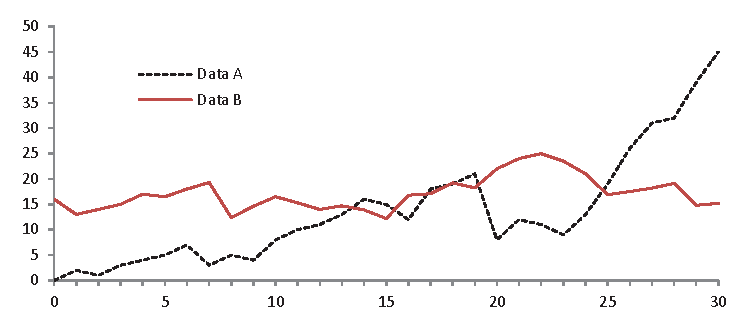
\includegraphics[width=\textwidth]{fig1.eps}
\caption{A figure caption is always placed below the illustration.
Please note that short captions are centered, while long ones are
justified by the macro package automatically.图标题需在图之后,且将所有图片放到与latex文件同路径的一个文件夹中} \label{fig1}
\end{figure}


引用参考文献
For citations of references, we prefer the use of square brackets
and consecutive numbers. Citations using labels or the author/year
convention are also acceptable. The following bibliography provides
a sample reference list with entries for journal
articles~\cite{ref_article1}, an LNCS chapter~\cite{ref_lncs1}, a
book~\cite{ref_book1}, proceedings without editors~\cite{ref_proc1},
and a homepage~\cite{ref_url1}. Multiple citations are grouped
\cite{ref_article1,ref_lncs1,ref_book1},
\cite{ref_article1,ref_book1,ref_proc1,ref_url1}.
%
% ---- Bibliography ----
%
% BibTeX users should specify bibliography style 'splncs04'.
% References will then be sorted and formatted in the correct style.
%
% \bibliographystyle{splncs04}
% \bibliography{mybibliography}
%
可直接去谷歌学术找到文献,直接下载latex信息用以复制粘贴到这里
\begin{thebibliography}{8}
\bibitem{ref_article1}
Author, F.: Article title. Journal \textbf{2}(5), 99--110 (2016)

\bibitem{ref_lncs1}
Author, F., Author, S.: Title of a proceedings paper. In: Editor,
F., Editor, S. (eds.) CONFERENCE 2016, LNCS, vol. 9999, pp. 1--13.
Springer, Heidelberg (2016). \doi{10.10007/1234567890}

\bibitem{ref_book1}
Author, F., Author, S., Author, T.: Book title. 2nd edn. Publisher,
Location (1999)

\bibitem{ref_proc1}
Author, A.-B.: Contribution title. In: 9th International Proceedings
on Proceedings, pp. 1--2. Publisher, Location (2010)

\bibitem{ref_url1}
LNCS Homepage, \url{http://www.springer.com/lncs}. Last accessed 4
Oct 2017
\end{thebibliography}
\end{document}
